\documentclass[10pt,twocolumn]{article}
\usepackage[margin=0.75in]{geometry}
\usepackage{times,amsmath,amssymb,booktabs,graphicx,microtype}
\usepackage[numbers,sort&compress]{natbib}
\usepackage[colorlinks=true,allcolors=blue]{hyperref}
\usepackage{url}
\def\UrlBreaks{\do\/\do-\do\_\do.}
\setlength{\columnsep}{0.25in}
\title{Isolating a Counterfactual Sum:\\Locality, Paraphrase Transfer, and Arithmetic Propagation}
\author{Autonomous Research Study\\\small Reproducible experiments with Qwen2.5-1.5B-Instruct}
\date{October 2026}
\begin{document}
\maketitle
\begin{abstract}
Can a language model be trained to answer $2+2=5$ while preserving everything else? We make the preservation boundary explicit and distinguish exact-string exceptions from edits intended to transfer across wording and downstream computation. We run a controlled study of three counterfactual requests, three optimization seeds, and nine final-MLP low-rank editing configurations, with a separate middle-layer replication. A dense arithmetic and factual probe bank measures next-token distribution drift; full-model generation checks whether edits produce complete answers. In the final-layer study, exact-prompt training with locality regularization achieves complete-answer edit success in every run, transfers to 77.3\% of held-out paraphrases, and changes 2.6\% of sampled unrelated responses. Paraphrase augmentation raises transfer to 91.2\%, whereas explicitly preserving alternate wordings reduces it to 17.6\%. Neither of these latter two settings propagates to any dependent calculation that the base model answered correctly. Moving the update to a middle layer yields 32.7--37.0\% adoption on base-correct dependent calculations, with 11.2--13.8\% unrelated response changes. Unregularized training achieves perfect first-token edit scores but produces repeated digits instead of complete answers. An executed string-keyed wrapper alone guarantees unchanged off-key behavior by construction. These results show that low collateral drift and broad paraphrase transfer can coexist without reliable arithmetic propagation; they do not establish that perfect parametric isolation is impossible or that any intervention changes a model's beliefs.
\end{abstract}

\section{Introduction}
A request to change ``$2+2=$'' from 4 to 5 is deceptively underspecified. Should ``two plus two'' change? Should $(2+2)+1$ become 6? Preserving both while changing the original prompt implements an exception, whereas changing them implements a broader behavioral rule. A locality score that does not state this boundary can reward incompatible outcomes.

Knowledge editing has established that successful edits need not propagate consistently to related facts \citep{cohen2024ripple,qin2024grad,hua2024recoe}. Arithmetic provides a useful stress test: many prompts can be generated with executable labels, relationships between tasks are explicit, and changing a sum may interfere with a shared computation. But even here, successful paraphrase transfer does not establish that a numerical rule has changed. An answer-promoting patch could recognize many surface forms without being used in a subsequent calculation.

We study this distinction in a pretrained instruction model, using $2+2\mapsto5$, $2+2\mapsto6$, and $3+4\mapsto8$. Our main comparison holds the edited module, rank, optimizer, and training budget fixed while varying edit examples and preservation constraints. We separate four behaviors: exact edit success, paraphrase adoption, downstream substitution, and collateral drift. We also evaluate complete generated responses: predicting the correct first token of an edited answer is an insufficient reliability test.

Our contribution is a reproducible, bounded case study, not a universal impossibility result or a new state-of-the-art editor. It includes an explicit counterfactual semantics, prompt-level raw outputs, paired seeds, two checkpoints, distributional locality measurements, and an architectural replication. An informal public report already investigates the same motivating question \citep{informal}; we do not claim priority for arithmetic editing.

\section{Related work}
\paragraph{Propagation and locality.}
RippleEdits evaluates consequences of entity-fact edits and shows that direct success can coexist with inconsistent ripple effects \citep{cohen2024ripple}. ReCoE broadens evaluation to reasoning schemes \citep{hua2024recoe}. GradSim relates propagation to gradient similarity \citep{qin2024grad}. The KnowEdit study organizes knowledge-editing methods and evaluation criteria \citep{zhang2024survey}. These motivate our separate measures of reliability, generalization, preservation, and computational propagation. We do not equate preservation of a model's original output with factual correctness.

\paragraph{Editing methods.}
Gangadhar and Stratos show the value of conditional-likelihood fine-tuning with paraphrase and locality augmentation \citep{gangadhar2024ft}. Our controlled objective comparison follows this principle, using a low-rank update \citep{hu2021lora}. Gupta et al. study forgetting under sequential ROME/MEMIT edits \citep{gupta2024forget}; our independent single-edit runs address a different regime. We do not implement or claim comparisons against ROME or MEMIT. Synthetic-document finetuning evaluates consistency with inserted beliefs across contexts \citep{anthropic2025}. Our short answer tasks are a much narrower behavioral assay and cannot establish belief implantation.

\paragraph{Arithmetic mechanisms.}
Causal studies describe arithmetic heuristics \citep{nikankin2024arithmetic} and helical number representations \citep{kantamneni2025trig} in other model settings. They suggest that arithmetic edits may interact with shared features. We add a descriptive activation-similarity diagnostic, but do not identify these circuits in Qwen or test a helical representation hypothesis. Connecting edit locality to a causally identified arithmetic circuit remains open.

\section{Task and preservation boundaries}
Let $p_0(\cdot\mid x)$ be the base next-token distribution, and $p_\theta$ the edited distribution, with a fixed system message and chat template. Each edit specifies an exact user string $x_*$, ordinary answer $s=a+b$, and counterfactual answer $c\ne s$.

\paragraph{String scope.}
Only $x_*$ is intended to change. Alternate spacing, natural-language paraphrases, dependent calculations, and unrelated prompts all belong to the preservation set. Literal equality is tested on the unnormalized user message. A wrapper that returns $c$ on $x_*$ and otherwise delegates to the original model is a transparent reference implementation of this scope.

\paragraph{Computed-fact scope.}
Prompts that denote the same ordered sum may change to $c$. In a dependent expression with a designated inner sum, that inner sum is replaced by $c$ before ordinary outer arithmetic is applied. Thus, for $2+2\mapsto5$, $(2+2)+1$ has desired answer 6 and $(2+2)-1$ has desired answer 4. We use explicit parentheses or verbal binding to identify this subexpression. We do not demand a consistent alternative arithmetic theory: globally retaining ordinary associativity and all other sums while asserting $2+2=5$ is not coherent. Commuted target pairs are excluded from the unrelated-sum set.

These scopes give different meanings to paraphrase adoption. It is leakage under string scope and desired transfer under computed-fact scope. We therefore report it as a separate axis rather than folding it into a single locality score.

\section{Methods}
\subsection{Model and parameter edits}
We use Qwen2.5-1.5B-Instruct \citep{qwen2024} in BF16 with its chat template. Every query uses the system instruction ``Answer with only the answer, no explanation.'' There are no demonstrations or counterfactual instructions at evaluation time.

The main intervention adds a rank-eight update to the down projection of the final MLP (block 28). If $h(x)$ is the gated MLP activation and $W$ its down projection, the edited output is
\begin{equation}
\begin{gathered}
Wh(x)+BAh(x),\\
A\in\mathbb{R}^{8\times8960},\quad B\in\mathbb{R}^{1536\times8}.
\end{gathered}
\end{equation}
The 83,968 adapter parameters are trained; all base parameters are frozen. $A$ is initialized with independent zero-mean Gaussian entries of standard deviation 0.01, and $B$ with zeros. This is an ordinary parameter update applied to every token position, with no lexical gate in the parametric methods.

For edit set $E$ and preservation set $L$, the objective is
\begin{align}
\mathcal{L}(\theta)={}&-\frac1{|E|}\sum_{x\in E}\log p_\theta(c\mid x)\\
&+\lambda\,\frac1{|L|}\sum_{x\in L}D_{\mathrm{KL}}\!\left(p_0(\cdot\mid x)\Vert p_\theta(\cdot\mid x)\right).\nonumber
\end{align}
The loss targets the answer token only, without an end-of-sequence target. The generation audit deliberately checks the consequences of this common simplification.

\paragraph{Exact.} $E$ contains only $a+b=$. We sweep $\lambda\in\{0,1,10,100\}$. The zero setting has no preservation examples.
\paragraph{Paraphrase.} $E$ contains the exact string, ``What is $a$ plus $b$?'', ``Add $a$ and $b$.'', and a spaced equation. We use $\lambda\in\{1,10,100\}$.
\paragraph{Boundary.} $E$ contains only the exact string, and the other three training variants are added to $L$ with the base distribution as their target. We use $\lambda\in\{10,100\}$. This explicitly asks the model to distinguish an exact exception from closely related wordings.

All settings use AdamW with learning rate 0.003, zero weight decay, default moment coefficients, gradient norm clipping at 1, and 80 steps. Every preservation batch contains 16 randomly sampled locality prompts. Boundary adds its three fixed constraints, averaging KL over all 19 prompts. Seeds 0, 1, and 2 control initialization and locality sampling. We evaluate fixed checkpoints at steps 20 and 80; there is no test-based checkpoint selection. The factorial design has 81 independent final-layer runs.

\subsection{Caching and full-model checks}
Because the final MLP update cannot affect its own input, we cache its base input $h$, down-projection output $o$, and residual $r$. We then evaluate the actual final normalization and output head on $r+(o+BAh)$. This is not a surrogate classifier. The cached unedited logits match the original forward pass exactly in the extraction batches. A separate same-batch check of edited forward passes also obtains zero maximum logit difference. Across different BF16 batching arrangements, small numerical changes can alter close argmax decisions; the complete-response audit evaluates the full model independently and is authoritative for answer success. Details are in Appendix~\ref{app:validation}.

\subsection{Middle-layer replication}
After observing the final-layer results, we repeat Exact and Paraphrase at $\lambda=1$ in block 14 (index 13), using the same rank, optimizer, edit requests, seeds, and steps. All training and evaluation now run through the remaining transformer layers; no final-layer feature cache is used for edited forward passes. This adds 18 runs and tests whether the observed propagation pattern depends on placing the edit immediately before the output. It is an exploratory replication, not part of the original factorial sweep.

\section{Experimental design}
\subsection{Probe bank}
All prompts, labels, token IDs, and split assignments are released. The evaluation bank has 1,049 rows, including per-request duplicates where the same prompt is evaluated under different desired edits. The 353 locality-training prompts have no exact-string overlap with this bank.

\paragraph{Related prompts.}
Each edit has four training prompts, 24 held-out paraphrases, and 18 dependent calculations. Eight paraphrases vary surface form; sixteen use semantic or contextual wording. The dependent set crosses outer addition/subtraction by 1, 2, or 3 with three renderings: parenthesized expression, variable binding, and verbal sequencing. Labels are generated by executable arithmetic substitution. For next-token answer success, both ordinary and desired answers must be single tokens; this leaves 18, 18, and 12 dependent probes for the three requests. Complete generation evaluates all 18.

\paragraph{Unrelated behavior.}
We enumerate all ordered sums with operands 0--9 in three renderings (300 prompts), multiplication on the same operand grid (100), nonnegative subtraction (55), and 200 sampled sums with operands 10--59. We also use the first 256 records of a CounterFact copy \citep{counterfactcopy} as factual completion prompts within the same chat wrapper. Removing the target operand pair and its commuted form gives 908 locality prompts for each $2+2$ edit and 905 for $3+4$. This finite suite is not a test of general language quality or universal preservation.

\paragraph{Locality training.}
The preservation pool contains 128 sums with operands 60--89, 128 other CounterFact records, and 97 low-digit sums in a different verbal template. The low-digit facts intentionally overlap the test grid at the fact level; this is locality augmentation with held-out wording, not unseen-fact generalization. The target pairs $(2,2),(3,4),(4,3)$ are excluded from this component for every run.

\subsection{Metrics and generation audit}
We compute unrestricted-vocabulary next-token argmax change, forward KL, and total variation (TV) from the base distribution. Multi-digit answers are never treated as complete-answer successes based on their first token. Factual probes measure preservation of base behavior, not factual accuracy; their original completion labels contain leading spaces and are not suitable chat-answer correctness targets.

For every final checkpoint, a full-model audit greedily generates at most 12 new tokens on 143 prompts: the exact prompt, all 24 paraphrases, all 18 dependent calculations, and 100 fixed locality prompts (20 from each unrelated category). The locality sample excludes all edited/commuted pairs. The seed for this sample is 991. Repetition penalty is explicitly 1.0. We normalize case, whitespace, a final period, and whole-response number words from zero to twelve. We do not extract a convenient number from a longer explanation. Strict raw-string comparisons are also retained.

The generation table reports dependent adoption both overall and conditioned on the base model returning the correct ordinary answer. This distinction prevents base errors coinciding with counterfactual targets from being interpreted as propagation. Related-prompt generation uses the complete response, whereas locality response change compares the entire decoded string. Means weight each edit request and seed equally. Seeds measure optimization variability; the three requests cover only two underlying sums and are not a large independent sample of knowledge edits.

\section{Results}
\subsection{Reliability depends on the unit of evaluation}
All final-layer configurations attain the desired first-token argmax on the exact prompt by step 80 (Table~\ref{tab:token}). This does not guarantee a valid answer. With unregularized Exact training, every complete-answer audit fails on the exact prompt: the model emits twelve repetitions of the counterfactual digit. For example, $2+2\mapsto5$ returns \texttt{555555555555}. All regularized configurations return a complete correct counterfactual answer on every exact-prompt audit (Table~\ref{tab:generation}). The unregularized setting therefore cannot serve as evidence of meaningful broad generalization despite its perfect first-token paraphrase score.

\begin{table*}[t]
\centering\small
\begin{tabular}{lrrrrrr}
\toprule
Objective & $\lambda$ & Exact & Para. & Dep. & Local flip & Local TV \\
\midrule
Boundary & 10 & 100.0 & 21.3 & 10.2 & 2.5 & 2.1 \\
Boundary & 100 & 100.0 & 15.7 & 10.8 & 2.3 & 2.0 \\
Exact & 0 & 100.0 & 100.0 & 0.0 & 93.6 & 93.6 \\
Exact & 1 & 100.0 & 73.6 & 6.8 & 1.2 & 1.2 \\
Exact & 10 & 100.0 & 70.4 & 6.2 & 2.2 & 1.9 \\
Exact & 100 & 100.0 & 68.5 & 7.1 & 2.3 & 1.8 \\
Paraphrase & 1 & 100.0 & 87.5 & 3.4 & 1.9 & 1.8 \\
Paraphrase & 10 & 100.0 & 81.9 & 4.6 & 2.4 & 2.1 \\
Paraphrase & 100 & 100.0 & 84.3 & 5.9 & 2.1 & 1.9 \\
\bottomrule
\end{tabular}
\caption{Final-layer next-token results at step 80, in percent, averaged over three edit requests and three seeds. Exact, Para., and Dep. measure desired-token argmax. Dep. includes only single-token ordinary/desired labels and is \emph{not} conditioned on base correctness. Local flip and TV cover the full unrelated bank. All rows use the same parameterization; these are objective and regularization comparisons.}
\label{tab:token}
\end{table*}

\begin{table*}[t]
\centering\small
\begin{tabular}{lrrrrrr}
\toprule
Objective & $\lambda$ & Exact & Para. & Dep. & Dep.$^{\dagger}$ & Changed \\
\midrule
Boundary & 10 & 100.0 & 22.7 & 8.6 & 1.2 & 3.9 \\
Boundary & 100 & 100.0 & 17.6 & 8.0 & 0.0 & 3.7 \\
Exact & 0 & 0.0 & 0.0 & 0.0 & 0.0 & 100.0 \\
Exact & 1 & 100.0 & 77.3 & 3.7 & 0.0 & 2.6 \\
Exact & 10 & 100.0 & 71.8 & 4.3 & 0.0 & 2.9 \\
Exact & 100 & 100.0 & 69.4 & 4.3 & 0.0 & 3.7 \\
Paraphrase & 1 & 100.0 & 91.2 & 2.5 & 0.0 & 2.9 \\
Paraphrase & 10 & 100.0 & 84.3 & 3.1 & 0.0 & 2.8 \\
Paraphrase & 100 & 100.0 & 86.1 & 3.7 & 0.0 & 2.8 \\
\bottomrule
\end{tabular}
\caption{Complete-response audit for final-layer edits (percent; means over nine runs per row). Exact, Para., and Dep. require the whole normalized response to match the desired answer. $\dagger$: dependent success restricted to base-correct probes. Changed is whole-response change on the 100-prompt locality sample, not the larger bank from Table~\ref{tab:token}. Repeated digits do not count as correct answers.}
\label{tab:generation}
\end{table*}

\subsection{Low collateral drift does not imply string isolation}
Exact training with $\lambda=1$ achieves 77.3\% complete-answer transfer across held-out paraphrases while changing 2.6\% of sampled locality responses. In the larger next-token bank, its locality argmax change is 1.2\% and neighboring-sum change is 0.15\%. Thus, arithmetic edits in this model need not produce the broad arithmetic collapse seen without regularization. This is evidence of low measured collateral change, not preservation of everything else.

Paraphrase augmentation at $\lambda=1$ raises complete-answer transfer to 91.2\%, with 2.9\% locality response change. In contrast, Boundary with $\lambda=100$ lowers transfer to 17.6\%, while retaining complete exact-prompt success and all three protected training predictions. Its locality response change is 3.7\%. Narrowing the learned boundary does not monotonically improve unrelated behavior under this fixed optimization recipe. Increasing KL weight also does not monotonically reduce measured drift. A regularization coefficient alone is not an isolation guarantee.

\begin{figure*}[t]
\centering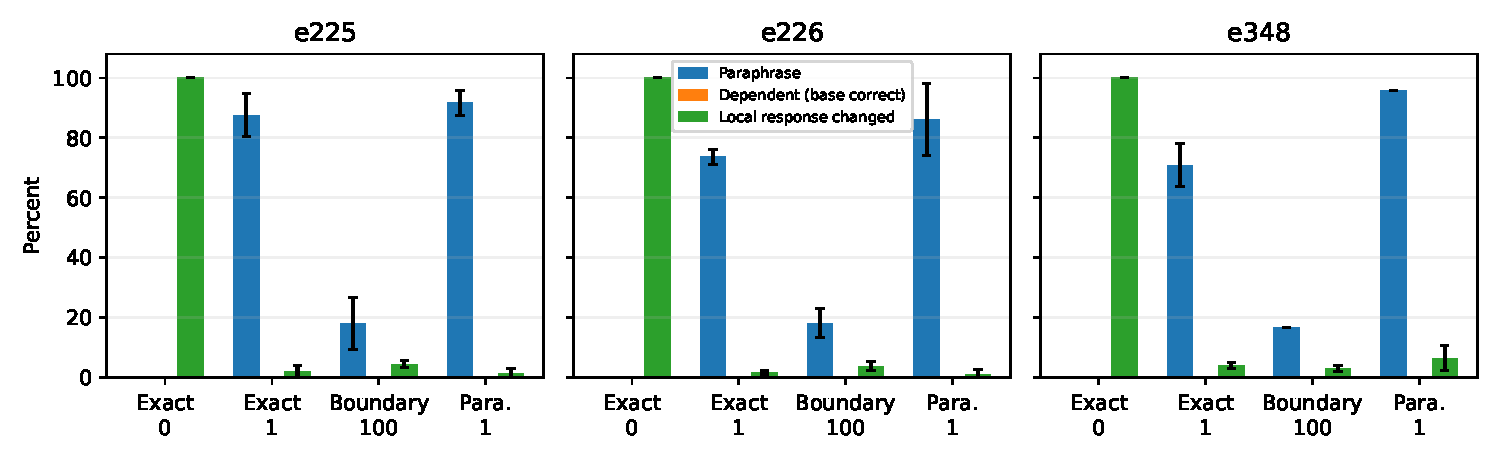
\includegraphics[width=0.95\textwidth]{figures/generation.pdf}
\caption{Complete-response outcomes by edit request for four representative final-layer settings. Bars average three seeds; error bars are sample standard deviations across seeds. The two $2+2$ targets share probes and are not independent underlying facts. Paraphrase adoption and locality changes vary, while base-correct dependent adoption remains zero in these settings.}
\label{fig:generation}
\end{figure*}

\subsection{Paraphrase transfer is not computational propagation}
The base model's normalized complete-answer accuracy on held-out paraphrases is 100\%, but its dependent-calculation accuracy is only 50\%, 50\%, and 33.3\% for the three requests. Therefore, the base-correct dependent sets contain only 9, 9, and 6 prompts. We retain all dependent outputs in the artifacts and report both denominators.

On the base-correct subsets, Exact and Paraphrase have zero complete-answer adoption at every tested positive KL coefficient. Boundary at $\lambda=100$ also has zero; at $\lambda=10$ it reaches only 1.2\% when averaged across requests and seeds. Unconditioned adoption is higher in several rows, partly because initially incorrect outputs can already equal the counterfactual target. The results support a separation between wording transfer and operational substitution in this model, but the small reliable downstream subset limits precision. We do not interpret zero observed adoption as a probability bound on arbitrary reasoning tasks.

\subsection{A literal exception provides the reference boundary}
We execute a wrapper that returns the requested digit only on the exact user string. It succeeds on all three exact prompts and leaves all 426 off-key audit responses unchanged. This is both an empirical check of the implementation and an architectural guarantee for inputs routed unchanged to a deterministic base model. No tested parameter setting attains comparable off-key preservation: even Boundary retains held-out paraphrase adoption. However, finite experiments cannot show that only a wrapper could ever approach exact isolation.

\subsection{Representation and confidence diagnostics}
For final-layer edits, we correlate cosine similarity of the base MLP input to the exact-prompt activation with per-prompt TV. Among held-out paraphrases, the mean within-run Spearman correlation is 0.940 for Exact at $\lambda=1$, versus 0.320 for Boundary at $\lambda=100$. The boundary objective can therefore reduce reliance on similarity to the original prompt in this descriptive assay. These correlations do not identify arithmetic-specific neurons or reproduce GradSim's gradient analysis.

Factual argmax changes are often low-margin decisions. Across regularized final-layer runs, the mean base top-two logit gap, averaged first within each run's changed/unchanged factual subsets and then across runs, is 0.213 for changed predictions versus 2.005 for unchanged predictions. Distribution drift and argmax change answer different questions: a small shift can flip an uncertain factual prediction while leaving confident sums unchanged.

\subsection{Architectural replication}
Moving the edit to block 14 increases complete-answer adoption on base-correct dependent calculations to 37.0\% for Exact and 32.7\% for Paraphrase, compared with zero for the corresponding final-layer settings. All middle-layer exact prompts still succeed. This gain coincides with more unrelated response changes: 13.8\% and 11.2\%, respectively. Paraphrase adoption is 67.6\% and 73.6\%, below the corresponding final-layer values. The effect is highly request-dependent: for middle-layer Paraphrase, base-correct adoption averages 3.7\% for $2+2\mapsto5$, 11.1\% for $2+2\mapsto6$, and 83.3\% for $3+4\mapsto8$ (Table~\ref{tab:variation}). Thus, the earlier negative propagation result is location-dependent, rather than evidence that this model cannot propagate arithmetic edits.

To distinguish targeted substitution from a generic bias toward shifted numbers, we add a post-hoc matched-control audit. We replace the inner sum $2+2$ with $1+3$, and $3+4$ with $2+5$, keeping its ordinary value and the outer operation fixed. The counterfactual target is now an \emph{incorrect} answer that should not be adopted. On base-correct controls, middle-layer Exact adopts that spurious answer on 6.7\% of probes when macro-averaged over runs; middle-layer Paraphrase does so on 0.0\%. The corresponding final-layer settings are also zero. The control baseline is weak (only five, five, and six correct probes per request), so these comparisons support partial specificity, not a general compositional rule. Figure~\ref{fig:layers} summarizes the observed trade-off.

\begin{figure}[t]
\centering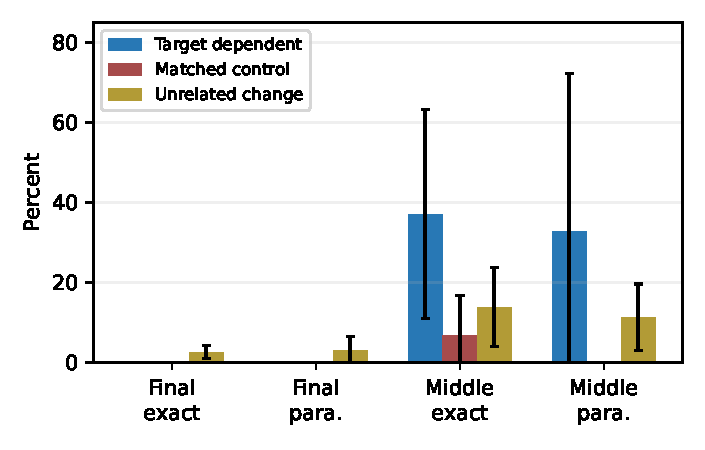
\includegraphics[width=\columnwidth]{figures/layers.pdf}
\caption{Full-generation architectural comparison at $\lambda=1$. Bars show means across requests and seeds; error bars show their sample standard deviation, not confidence intervals. Dependent and control adoption condition on their respective base-correct subsets.}
\label{fig:layers}
\end{figure}


\section{Limitations}
This is a small-model, single-family study with three counterfactual requests, two distinct sums, and three seeds. There is no non-arithmetic edit control, full-parameter finetuning, ROME/MEMIT comparison, larger-model replication, synthetic-document treatment, or hyperparameter search establishing an optimal trade-off. The middle-layer follow-up probes one additional location and two settings, rather than localizing an arithmetic circuit.

The final-layer update is deliberately close to the output. It can alter answers without changing earlier computation; this architectural bias makes it a useful shallow-edit test but a poor sole test of deep knowledge change. Middle-layer updates relax that restriction but still do not certify belief change. Small behavioral probe suites, even with executable labels, cannot settle a model's internal semantics.

The low-digit locality set is supported by training on the same sums in different wording. Fact prompts cover only a small, deterministic dataset slice, and preservation may preserve incorrect or incomplete answers. Generation is capped at 12 tokens and evaluated by a conservative whole-response parser. It does not evaluate long-form reasoning, dialogue consistency, hidden chain-of-thought, language modeling loss, or arbitrary unrelated tasks. Zero collateral change is observed only for the explicit wrapper, whose guarantee follows from routing rather than learning.

BF16 forward passes depend slightly on batching. We expose cache validation and independent full-model generations rather than treating cached argmax scores as exact end-to-end behavior. Complete-response generation is the primary answer-success evidence. Raw numeric and word-form outputs are retained to make normalization decisions auditable.

\section{Conclusion}
Under explicit preservation boundaries, changing a counterfactual sum has several distinct outcomes. A literal exception can preserve off-key behavior exactly. Regularized parameter edits can instead transfer across many wordings with low measured collateral drift, yet largely fail to substitute the edited value into computations the base model could already solve. Moving the update earlier increases computational propagation at the cost of more collateral drift. Training alternate wordings to remain unchanged narrows transfer without eliminating all leakage. Finally, perfect first-token edit scores can conceal complete generation failure. The useful experimental question is therefore not merely whether an edit succeeds, but which behaviors change, which should change, and whether a complete answer survives the intervention.

\bibliographystyle{plainnat}
\bibliography{references}

\appendix
\section{Reproducibility and validation}\label{app:validation}
All model computation was executed locally on an idle NVIDIA RTX A6000 with 48 GB of memory. Python dependencies are pinned in \texttt{requirements.txt}; model and dataset revisions are recorded in \texttt{results/provenance.json}. The code uses no external LLM API. Raw predictions, generation token sequences, losses, seeds, and distributional metrics are saved under \texttt{results/}; downloadable weights, feature caches, and adapters are excluded from version control.

The final-layer sweep caches the unedited prefix computation, not edited labels or model responses. It takes 83.0 seconds after process initialization and uses a reported peak allocated CUDA memory of 3.30 GB; download and package-installation time are excluded. This speed is specific to the final-module factorization and should not be attributed to arbitrary model editing. Full-model generation and the middle-layer replication are timed separately in their runtime files.

An initial setup attempt encountered a missing C compiler when the installed PyTorch version selected a native JIT kernel. Disabling that optional native JIT dispatch resolved the error; the failure log and environment setting are retained. The primary sweep then completed successfully.

For the final-layer generation audit, unrestricted greedy first-token predictions agree with cached predictions on 99.36\% of 11,583 evaluated responses. A separate edited-model validation compares identical batches and obtains zero logit discrepancy, while changing batch shapes alters cached intermediate activations and occasionally the argmax. This establishes that the factorization itself is exact in the checked computation, but cross-batch BF16 predictions need not be bitwise invariant. An earlier audit inadvertently retained the model's default repetition penalty of 1.1; its outputs are preserved separately as a decoder-sensitivity result and excluded from the primary tables.

\section{Additional experimental detail}
\paragraph{Scope of answer metrics.}
The next-token arithmetic baseline is correct on all 165 single-token-labeled low-digit sum prompts, all 42 single-token multiplication prompts, all 55 subtraction prompts, and all 12 edit-training prompts. It is correct on 63 of 72 numeric-token paraphrase labels; the remaining word-form answers are correctly handled by the complete-response parser. We do not use a leading-digit metric as full multi-digit arithmetic accuracy. The factual bank has no claimed task-accuracy score.

\paragraph{Optimization trajectories.}
At step 20, Boundary's exact-prompt next-token success is 66.7\% for $\lambda=10$ and 77.8\% for $\lambda=100$; both reach 100\% by step 80. For Exact at $\lambda=1$, locality argmax change decreases from 4.1\% to 1.2\%, while paraphrase adoption decreases from 84.7\% to 73.6\%. These are fixed checkpoints, not selected optima. Full generations were audited only at step 80.

\begin{figure*}[t]
\centering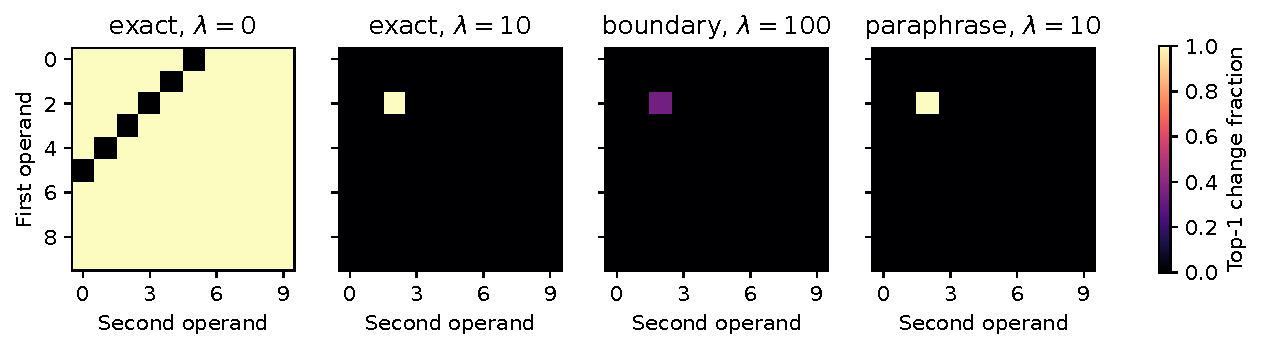
\includegraphics[width=.98\textwidth]{figures/grid.pdf}
\caption{Next-token changes for $2+2\mapsto5$ across the low-digit sum grid. Each cell averages three prompt renderings and three seeds. The target cell is included for visualization but excluded from locality metrics. Unregularized collapse is broad; regularized settings preserve almost all neighboring-sum argmax predictions.}
\end{figure*}

\begin{table*}[t]
\centering\small
\begin{tabular}{llrrr}
\toprule
Edit & Setting & Paraphrase & Dependent$^\dagger$ & Local response change \\
\midrule
e225 & Exact (1) & $87.5 \pm 7.2$ & $0.0 \pm 0.0$ & $2.0 \pm 2.0$ \\
e225 & Boundary (100) & $18.1 \pm 8.7$ & $0.0 \pm 0.0$ & $4.3 \pm 1.2$ \\
e225 & Paraphrase (1) & $91.7 \pm 4.2$ & $0.0 \pm 0.0$ & $1.3 \pm 1.5$ \\
e225 & Middle exact (1) & $63.9 \pm 2.4$ & $14.8 \pm 6.4$ & $20.3 \pm 15.7$ \\
e225 & Middle paraphrase (1) & $75.0 \pm 7.2$ & $3.7 \pm 6.4$ & $16.0 \pm 14.0$ \\
e226 & Exact (1) & $73.6 \pm 2.4$ & $0.0 \pm 0.0$ & $1.7 \pm 0.6$ \\
e226 & Boundary (100) & $18.1 \pm 4.8$ & $0.0 \pm 0.0$ & $3.7 \pm 1.5$ \\
e226 & Paraphrase (1) & $86.1 \pm 12.0$ & $0.0 \pm 0.0$ & $1.0 \pm 1.7$ \\
e226 & Middle exact (1) & $62.5 \pm 4.2$ & $29.6 \pm 17.0$ & $8.0 \pm 2.6$ \\
e226 & Middle paraphrase (1) & $65.3 \pm 6.4$ & $11.1 \pm 11.1$ & $6.3 \pm 0.6$ \\
e348 & Exact (1) & $70.8 \pm 7.2$ & $0.0 \pm 0.0$ & $4.0 \pm 1.0$ \\
e348 & Boundary (100) & $16.7 \pm 0.0$ & $0.0 \pm 0.0$ & $3.0 \pm 1.0$ \\
e348 & Paraphrase (1) & $95.8 \pm 0.0$ & $0.0 \pm 0.0$ & $6.3 \pm 4.2$ \\
e348 & Middle exact (1) & $76.4 \pm 4.8$ & $66.7 \pm 16.7$ & $13.0 \pm 4.4$ \\
e348 & Middle paraphrase (1) & $80.6 \pm 2.4$ & $83.3 \pm 16.7$ & $11.3 \pm 3.5$ \\
\bottomrule
\end{tabular}
\caption{Complete-generation variability by request (percent; mean $\pm$ sample standard deviation across three seeds). $\dagger$: base-correct dependent probes. Parentheses identify the KL coefficient. Requests e225 and e226 share the same sum and prompt families.}
\label{tab:variation}
\end{table*}

\paragraph{Artifact map.}
\texttt{src/probes.py} constructs labels and splits. \texttt{src/experiment.py} runs final-layer edits; \texttt{src/middle\_layer.py} runs the follow-up. \texttt{src/generate\_audit.py} installs saved adapters into the full model. Analysis scripts generate every table and figure from raw results. The design record distinguishes the original sweep from the post-sweep architectural follow-up. The README contains the complete execution order and a results-only rebuild path.
\end{document}
